% +------------------------------------------------------------------------+
% | CGAL Reference Manual:  hds.tex
% +------------------------------------------------------------------------+
% | Combinatoric and geometry of polyhedral surfaces in 
% | halfedge representation.
% |
% | 11.10.1996   Lutz Kettner
% |              Start rewriting the whole stuff
% | 
\RCSdef{\hdsRev}{$Revision$}
\RCSdefDate{\hdsDate}{$Date$}
% +------------------------------------------------------------------------+

\ccParDims

\chapter{Halfedge Data Structures}
\label{chapterHds}
\ccChapterRelease{\hdsRev. \ \hdsDate}\\
\ccChapterAuthor{Lutz Kettner}


% +------------------------------------------------------------------------+
\section{Introduction}

A halfedge data structure is an edge-centered data structure capable
of maintaining incidence informations of vertices, edges and facets,
for example for planar maps, polyhedra, or other orientable,
two-dimensional surfaces embedded in arbitrary dimension. Each edge is
decomposed into two halfedges with opposite orientations. One incident
facet and one incident vertex are stored in each halfedge.  For each
facet and each vertex one incident halfedge is stored.  Reduced
variants of the halfedge data structure can omit some of these
informations, for example the halfedge pointers in vertices or the
storage of vertices at all.

\begin{ccTexOnly}
    \vspace{-4mm}
    \begin{center}
      \parbox{0.4\textwidth}{%
          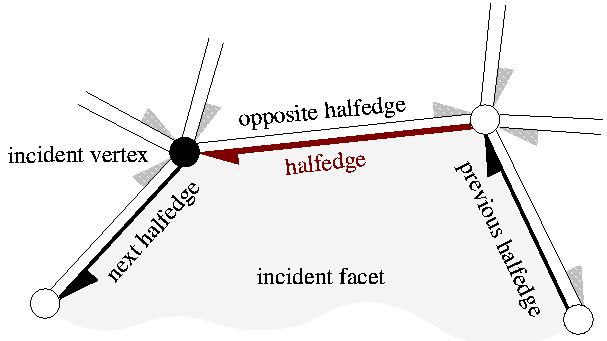
\includegraphics[width=0.4\textwidth]{idraw/halfedge.ips}%
      }
    \end{center}
    \vspace{-3mm}
\end{ccTexOnly}

\begin{ccHtmlOnly}
    <CENTER>
    <A HREF="./halfedge.gif">
        <img src="./halfedge_small.gif" alt="Halfedge Diagram"></A><P>
    </CENTER>
\end{ccHtmlOnly}

The data structure provided here is known as the
FE-structure~\cite{w-ebdss-85}, as
halfedges~\cite{m-ism-88,bfh-mgedm-95} or as the doubly connected edge
list (DCEL)~\cite{bkos-cgaa-97}, although the original reference for
the DCEL~\cite{mp-fitcp-78} describes a different data structure. We
continue naming it halfedge data structure (HDS). This data structure
can also be seen as one of the variants of the quad-edge data
structure~\cite{gs-pmgsc-85}, reduced to support only orientable
surfaces. In general, the quad-edge data structure has a richer
modeling space and can represent non-orientable 2-manifolds. The dual
and the primal graph are symmetrically represented; the same
algorithms can be applied to the dual graph as well as to the primal
graph. This implies a lack of static type checking to distinguish
between facets and vertices.  Even though halfedges are similar to the
winged edge data structure~\cite{b-prcv-75} or the original reference
for the DCEL~\cite{mp-fitcp-78}, they are not equivalent, since the
traversal algorithms are forced to search for certain incidences where
the information is directly available in the halfedge data structure.
An overview and comparison of these different data structures together
with a thorough description of the design implemented here can be
found in~\cite{k-ddsps-98}.


\subsection*{Design Overview}

The design strictly separates topology and geometry. Vertices,
halfedges and facets carry both kinds of information. The
\ccc{Halfedge_data_structure} acts as a container class and stores all
items and manages their incidence relations. For example the
\ccc{Polyhedron} from Chapter~\ref{chapterPolyhedron} uses the
\ccc{Halfedge_data_structure} and adds geometric operations. It
imposes further restrictions on the data structure, for example, that
an edge always has two distinct endpoints.


\begin{ccTexOnly}
  \begin{figure}
    \begin{center}
      \parbox{0.7\textwidth}{%
          \includegraphics[width=0.7\textwidth]{idraw/poly_design.ips}%
      }
    \end{center}
    \caption{Responsibilities of the different layers in the 
             halfedge data-structure design.}
    \label{figurePolyDesign}
  \end{figure}
\end{ccTexOnly}

\begin{ccHtmlOnly}
    <CENTER>
    <A NAME="figurePolyDesign">
        <img src="./poly_design_color.gif"
         alt="Halfedge Data-Structure Design"><BR>
    Figure: Responsibilities of the different layers in the 
            halfedge data-structure design.
    <P>
    </CENTER>
\end{ccHtmlOnly}

Figure~\ccTexHtml{\ref{figurePolyDesign}}{}\begin{ccHtmlOnly}
  <A HREF="Chapter_hds.html#figurePolyDesign"><IMG 
  SRC="cc_ref_up_arrow.gif" ALT="reference arrow" WIDTH="10" HEIGHT="10"></A>
\end{ccHtmlOnly}
offers a closer look at the design using \ccc{Polyhedron} as example.
Note that \ccc{Halfedge_data_structure}, \ccc{Vertex_base}, \ccc{Halfedge_base}
and \ccc{Facet_base} are concepts, where each can have multiple
models. There are many different possibilities for vertices, edges and
facets. Currently, two different models are provided for the
\ccc{Halfedge_data_structure}. Many combinations are possible and
result in a different \ccc{Polyhedron}.  We make use of the
implicit instantiation of template classes in \CC.  The requirement
set for a model consists of a mandatory part that every model must
comply with and certain optional parts a model must only comply with
if the corresponding functionality is actually used. For example, a
vertex is allowed to be empty. If we want to use it for the polyhedral
surface, then the normal vector computation imposes the additional
requirements that the vertex must contain a three-dimensional point
and gives access to it with the member function \ccc{point()}.

The responsibilities of the base classes for vertices, halfedges and
facets are the actual storage of the incidences in terms of
\ccc{void}-pointers, the geometry and other attributes. Especially the
storage of incidences with \ccc{void}-pointers allows, for example,
the facet class to be exchanged without rewriting the halfedge class.
The advantage of strong type checking will be reestablished in the
next layer.  Implementations for vertices, edges and facets are
provided that fulfill the minimal set of requirements. They can be
used as base classes for own extensions.  Richer implementations are
provided as defaults; for polyhedra they provide a three-dimensional
point in the vertices and a plane equation in the facets.

The \ccc{Halfedge_data_structure} is responsible for the storage
organization of the vertices, halfedges and facets. Currently,
implementations are provided that use a bidirectional list or an \stl\ 
\ccc{std::vector} internally. The \ccc{Halfedge_data_structure} derives new
classes for vertices, halfedges and facets. They replace the
\ccc{void}-pointer incidence information with type-safe pointers at
the interface. Additional information besides the incidence
information simply stays unaffected and will be inherited.

Different models are possible for the \ccc{Halfedge_data_structure}
(two are available right now).  Thus the set of requirements for the
\ccc{Halfedge_data_structure} is kept small. To support the
implementation of high-level operations, a helper class
\ccc{Halfedge_data_structure_decorator} is provided, which is not
shown in Figure~\ccTexHtml{\ref{figurePolyDesign}}{}\begin{ccHtmlOnly}
  <A HREF="Chapter_hds.html#figurePolyDesign"><IMG 
  SRC="cc_ref_up_arrow.gif" ALT="reference arrow" WIDTH="10" HEIGHT="10"></A>
\end{ccHtmlOnly}
 but would be placed at the side
of the \ccc{Halfedge_data_structure}, since it broadens that interface
but does not hide it. It adds Euler operations and adaptive
functionality.  For example, if the \ccc{prev()} function is not
provided for halfedges, a \ccc{find_prev()} function searches the
previous halfedge along the facet. If the \ccc{prev()} function is 
available, the \ccc{find_prev()} function simply calls it. This
distinction is resolved at compile time with a technique called {\em
  compile-time tags}, similar to iterator tags in~\cite{sl-stl-95}.

The \ccc{Polyhedron} (Chapter~\ref{chapterPolyhedron}) adds an 
ease-of-use layer in terms of high-level
functions, high-level concepts for accessing the items, i.e.~handles,
iterators and circulators (pointers are no longer visible at this
interface), and the protection of the combinatorial integrity. It
derives new vertices, halfedges and facets to provide the handles and
hide the pointers.

\subsection*{Organization of this Chapter}

Section~\ref{sectionHds} describes the requirements a
\ccc{Halfedge_data_structure} with its three local classes for
vertices, halfedges and facets must fulfill.
Section~\ref{sectionHdsModels} names the models currently available.
These models make use of the \ccc{Vertex_base}, \ccc{Halfedge_base}
and \ccc{Facet_base} concepts, whose requirements are stated in
Section~\ref{sectionHdsBases}. The predefined base classes are
described in Section~\ref{sectionHdsBasesModels}. The helper class
\ccc{Halfedge_data_structure_decorator} follows in
Section~\ref{sectionHdsDecorator}. Several examples of halfedge data
structures in Section~\ref{sectionHdsExamples} conclude the chapter.


% +========================================================================+
\ccHtmlNoClassToc
\begin{ccClass}{Halfedge_data_structure}
\section{Requirements for a \protect\ccc{Halfedge_data_structure}}
% +========================================================================+
\label{sectionHds}
\ccCreationVariable{hds}
\def\ccTagRmTrailingConst{\ccFalse}

\ccDefinition  

A \ccClassTemplateName\ consists of vertices $V$, edges $E$, facets
$F$ and an incidence relation on them.  Each edge is represented by
two halfedges with opposite orientations. Vertices and facets are
optional. See 
Figure~\ccTexHtml{\ref{figureOptionalMethods}}{}\begin{ccHtmlOnly}
  <A HREF="Halfedge_data_structure.html#figureOptionalMethods"><IMG 
  SRC="cc_ref_up_arrow.gif" ALT="reference arrow" WIDTH="10" HEIGHT="10"></A>
\end{ccHtmlOnly}
 for the incidences
stored and the mandatory or optional member functions possible for
vertices, halfedges and facets.

\begin{ccTexOnly}
    \begin{figure}
        \begin{center}
          \parbox{\textwidth}{%
              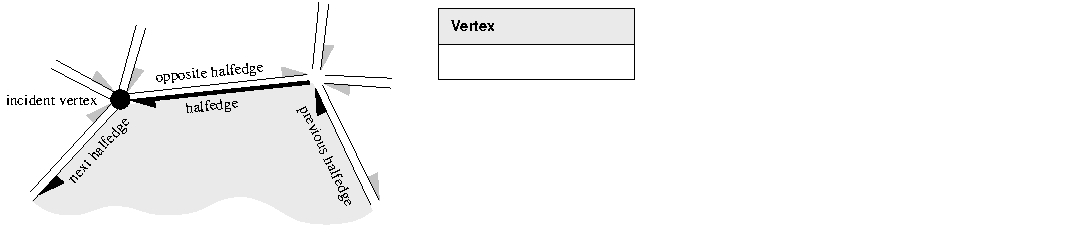
\includegraphics[width=\textwidth]{idraw/hds_optional.ips}%
          }
        \end{center}
        \caption{The three classes \protect\ccc{Vertex}, 
          \protect\ccc{Halfedge}, and 
          \protect\ccc{Facet} of the halfedge data structure. Member
          functions with shaded background are mandatory. The others
          are optionally supported.}
        \label{figureOptionalMethods}
    \end{figure}
\end{ccTexOnly}

\begin{ccHtmlOnly}
    <CENTER>
    <A NAME="figureOptionalMethods">
    <A HREF="./hds_optional.gif">
        <img src="./hds_optional_small.gif" 
             alt="Class Diagram"></A><BR>
    <A HREF="./hds_optional.gif">Figure:</A>
    The three classes <I>Vertex</I>, <I>Halfedge</I>, and 
          <I>Facet</I> of the halfedge data structure. Member
          functions with shaded background are mandatory. The others
          are optionally supported.
    </CENTER>
\end{ccHtmlOnly}

A model for the \ccClassName\ concept must provide the following types
and operations.  In addition, the local types \ccc{Vertex},
\ccc{Halfedge} and \ccc{Facet} must fulfill the requirements listed in
the Sections~\ref{sectionHdsVertex} to \ref{sectionHdsFacet}.


% +-----------------------------------+
\ccTypes

\ccThree{Halfedge_data_structure&}{hds.capofhalfedges() const;;}{}
\ccThreeToTwo

\ccNestedType{Vertex}{vertex type, model of \ccc{HDS_Vertex}.}
\ccGlue
\ccNestedType{Halfedge}{halfedge type, model of \ccc{HDS_Halfedge}.}
\ccGlue
\ccNestedType{Facet}{facet type, model of \ccc{HDS_Facet}.}
\ccGlue
\ccNestedType{Size}{type for size values.}
\ccGlue
\ccNestedType{Difference}{type for difference values.}


\ccNestedType{Point}{type for the (optionally) associated geometry for
  vertices. If no point geometry is supported, the type is \ccc{void*}.}

For the following iterators exist appropriate const iterators too.

\ccNestedType{Vertex_iterator}{iterator over all vertices.}
\ccGlue
\ccNestedType{Halfedge_iterator}{iterator over all halfedges.}
\ccGlue
\ccNestedType{Facet_iterator}{iterator over all facets.}
\ccGlue
\ccNestedType{iterator_category}{category for all iterators.}

% +-----------------------------------+
\ccCreation

\ccConstructor{Halfedge_data_structure();}
             {the empty data structure \ccVar.}

\ccConstructor{Halfedge_data_structure( Size v, Size h, Size f);}
              {a data structure \ccVar\ with storage reserved
               for $v$ vertices, $h$ halfedges, and $f$ facets. The
               reservation sizes are a hint for optimizing storage
               allocation.}


%\ccConstructor{Halfedge_data_structure( const Halfedge_data_structure&
%    hds2);}{copy constructor performing deep copy.}

%\ccMethod{Halfedge_data_structure& operator=( const
%    Halfedge_data_structure& hds2);}{assignment performing deep copy.}

\ccThree{Halfedge_iterator}{hds.reser}{}

\ccMethod{void reserve( Size v, Size h, Size f);}{reserves storage
               for $v$ vertices, $h$ halfedges, and $f$ facets. The
               reservation sizes are a hint for optimizing storage
               allocation. If the \ccc{capacity()} is already greater
               than the requested size nothing happens. If the
               \ccc{capacity} changes all iterators and circulators
               might be invalidated.}
\ccThree{Halfedge_iterator}{hds.capacity_of_halfedges() const;;}{}

% +-----------------------------------+
\ccHeading{Access Member Functions}


\def\ccTagRmConstRefPair{\ccFalse}
\def\ccTagRmEigenClassName{\ccFalse}


\ccMethod{Size size_of_vertices() const;}
    {number of vertices.}
\ccGlue
\ccMethod{Size size_of_halfedges() const;}
    {number of halfedges.}
\ccGlue
\ccMethod{Size size_of_facets() const;}
    {number of facets.}
\ccGlue
\ccMethod{Size capacity_of_vertices() const;}
    {space reserved for vertices.}
\ccGlue
\ccMethod{Size capacity_of_halfedges() const;}
    {space reserved for halfedges.}
\ccGlue
\ccMethod{Size capacity_of_facets() const;}
    {space reserved for facets.}
\ccGlue
\ccMethod{std::size_t bytes() const;}
    {bytes used for \ccVar.}
\ccGlue
\ccMethod{std::size_t bytes_reserved() const;}
    {bytes reserved for \ccVar.}
    
The following member functions return the non-mutable iterator or
non-mutable circulator respectively if the halfedge data structure
will be declared const.

\ccMethod{Vertex_iterator    vertices_begin();}{iterator over all vertices.}
\ccGlue
\ccMethod{Vertex_iterator    vertices_end();}{}
\ccGlue
\ccMethod{Halfedge_iterator  halfedges_begin();}{iterator over all halfedges}
\ccGlue
\ccMethod{Halfedge_iterator  halfedges_end();}{}
\ccGlue
\ccMethod{Facet_iterator     facets_begin();}{iterator over all facets.}
\ccGlue
\ccMethod{Facet_iterator     facets_end();}{}



% +-----------------------------------+
\ccHeading{Insertion}

The following operations  allocate a new element of the named item.
Halfedges are always allocated in pairs of opposite halfedges.
The opposite pointers are automatically set. Note that
\ccc{new_vertex()} and \ccc{new_facet()} might not be present for
halfedge data structures that do not support vertices or facets
respectively.

\ccMethod{Vertex* new_vertex();}{creates a default vertex.}
\ccGlue
\ccMethod{Vertex* new_vertex(const Vertex* v);}{creates a copy of $v$.}
\ccGlue
\ccMethod{Vertex* new_vertex(const Point& p);}{creates a new vertex
          initialized to $p$.}
\ccGlue
\ccMethod{Halfedge* new_edge();}{creates a new pair of opposite halfedges.}
\ccGlue
\ccMethod{Halfedge* new_edge(const Halfedge* h);}{creates a copy of
          the two halfedges $h$ and \ccc{h->opposite()}.}
\ccGlue
\ccMethod{Facet* new_facet();}{creates a default facet.}
\ccGlue
\ccMethod{Facet* new_facet(const Facet* f);}{creates a copy of $f$.}


% +-----------------------------------+
\ccHeading{Removal}

The following operations erase an element referenced by a pointer.
Halfedges are always deallocated in pairs of opposite halfedges,
however, the halfedge pointer might denote any of the two possible
halfedges.  Erasing single elements is optional and indicated with the
type tag \ccc{Supports_removal}. The \ccc{pop_back} member functions,
which remove the element that was created last, and the deletion of
all items are mandatory, if the corresponding item is supported.

\ccMethod{void delete_vertex( Vertex* v);}{deletes the vertex $v$.}
\ccGlue
\ccMethod{void delete_edge( Halfedge* h);}{deletes the pair of
          opposite halfedges $h$.} 
\ccGlue
\ccMethod{void delete_facet( Facet* f);}{deletes the facet $f$.}

\ccMethod{void vertex_pop_back();}{removes last vertex. Mandatory.}
\ccGlue
\ccMethod{void edge_pop_back();}{removes last pair of halfedges. Mandatory.}
\ccGlue
\ccMethod{void facet_pop_back();}{removes last facet. Mandatory.}
\ccGlue
\ccMethod{void delete_all();}{deletes all elements. Mandatory.}

% +-----------------------------------+
\ccHeading{Operations with Border Halfedges}

\begin{ccAdvanced}
  
The following notion of border halfedges is particularly useful
where the halfedge data structure is used to model surfaces with a
border. The halfedge data structure does not support holes within a
facet, but the surface can have open regions. Halfedges at the border
of the surface are called {\em border halfedges}. A halfedge is a {\em
  border edge\/} if the halfedge itself or its opposite halfedge are
border halfedges. The only requirement to work with border halfedges
is that the \ccc{Halfedge} class provides a member function
\ccc{is_border()} returning a \ccc{bool}. Usually, the halfedge data
structure supports facets and a \ccc{NULL} facet pointer will indicate
a border halfedge, but this is not the only possibility.  The
\ccc{is_border()} predicate divides the edges into two classes, the
border edges and the non-border edges. The following normalization
reorganizes the sequential storage of the edges such that the
non-border edges precede the border edges, and that for each border
edge the latter of the two halfedges is a border halfedge (the first
one might be a border halfedge too). The normalization stores the
number of border halfedges, as well as the halfedge iterator where the
border edges start at, within the halfedge data structure.  Halfedge
insertion or removal and changing the border status of a halfedge may
invalidate these values, which are not automatically updated.

\ccThree{Halfedge_iterator}{hds.size_of;}{}

\ccMethod{void   normalize_border();}
    {sorts halfedges such that the non-border edges precede the
     border edges. For each border edge that is incident to a facet,
     the halfedge iterator will reference the halfedge incident to the
     facet right before the halfedge that is not incident to a facet.}

\ccMethod{Size size_of_border_halfedges() const;}
    {number of border halfedges. An edge with no incident facet
      counts as two border halfedges.
    \ccPrecond \ccc{normalize_border()} has been called and no
    halfedge insertion or removal and no change in border
    status of the halfedges have occurred since then.}

\ccMethod{Size size_of_border_edges() const;}
    {number of border edges. If \ccc{size_of_border_edges()} is equal
    to \ccc{size_of_border_halfedges()} all border edges are incident to
    a facet on one side and to no facet on the other side.
    \ccPrecond \ccc{normalize_border()} has been called and no
    halfedge insertion or removal and no change in border
    status of the halfedges have occurred since then.}

\ccMethod{Halfedge_iterator  border_halfedges_begin();}
    {halfedge iterator starting with the border edges. The range
      [\ccStyle{halfedges_begin(), border_halfedges_begin()}) denotes
    all non-border edges. The range
    [\ccStyle{border_halfedges_begin(), halfedges_end()}) denotes all
    border edges.
    \ccPrecond \ccc{normalize_border()} has been called and no
    halfedge insertion or removal and no change in border
    status of the halfedges have occurred since then.}

\end{ccAdvanced}

% +-----------------------------------+
\ccHeading{Types for Tagging Optional Features}

\begin{ccAdvanced}

The nested types below are either equal to \ccStyle{Tag_true} or
\ccStyle{Tag_false}, depending on whether the named member function is
supported or not. Those related to vertices, halfedges and facets are
identical to the definitions for the local vertex, halfedge or facet
class respectively.

\ccNestedType{Supports_vertex_halfedge}{\ccc{Vertex::halfedge()}.}
\ccGlue
\ccNestedType{Supports_vertex_point}{\ccc{Vertex::point()}.}
\ccGlue
\ccNestedType{Supports_halfedge_prev}{\ccc{Halfedge::prev()}.}
\ccGlue
\ccNestedType{Supports_halfedge_vertex}{\ccc{Halfedge::vertex()}.}
\ccGlue
\ccNestedType{Supports_halfedge_facet}{\ccc{Halfedge::facet()}.}
\ccGlue
\ccNestedType{Supports_facet_halfedge}{\ccc{Facet::halfedge()}.}

\ccNestedType{Supports_removal}{the halfedge data structure
  supports the removal of individual elements of a surface, i.e.
  \ccc{delete_edge()}, \ccc{delete_vertex()} if vertices are supported, and
  \ccc{delete_facet()} if facets are supported.}

The following dependencies among these options must be regarded:

Vertices are supported $\Longleftrightarrow$
\ccc{Supports_halfedge_vertex} $\equiv$ \ccc{Tag_true}.
\\
Facets are supported $\Longleftrightarrow$
\ccc{Supports_halfedge_facet} $\equiv$ \ccc{Tag_true}.
\\
\ccc{Supports_vertex_halfedge} $\equiv$ \ccc{Tag_true} $\Longrightarrow$
\ccc{Supports_halfedge_vertex} $\equiv$ \ccc{Tag_true}.
\\
\ccc{Supports_vertex_point} $\equiv$ \ccc{Tag_true} $\Longrightarrow$
\ccc{Supports_halfedge_vertex} $\equiv$ \ccc{Tag_true}.
\\
\ccc{Supports_facet_halfedge} $\equiv$ \ccc{Tag_true} $\Longrightarrow$
\ccc{Supports_halfedge_facet} $\equiv$ \ccc{Tag_true}.

\end{ccAdvanced}

\ccSeeAlso

\ccc{Halfedge_data_structure_decorator} 
in Section~\ref{sectionHdsDecorator}.
\ccc{Polyhedron_3} 
in Chapter~\ref{chapterPolyhedron}.

\end{ccClass} %% Halfedge_data_structure



% +-------------------------------------------------------------+
\begin{ccClass}{HDS_Vertex}
\subsection{Requirements for a \protect\ccc{HDS_Vertex}}
\label{sectionHdsVertex}


% +-----------------------------------+
\ccDefinition

A vertex optionally stores a point and a pointer to an incident
halfedge that points to the vertex.  Type tags indicate whether these
member functions are supported.  
Figure~\ccTexHtml{\ref{figureOptionalMethods}}{}\begin{ccHtmlOnly}
  <A HREF="Halfedge_data_structure.html#figureOptionalMethods"><IMG 
  SRC="cc_ref_up_arrow.gif" ALT="reference arrow" WIDTH="10" HEIGHT="10"></A>
\end{ccHtmlOnly}
depicts the relationship between a halfedge and its incident halfedges,
vertices, and facets.

\ccCreationVariable{v}
\ccThree{Halfedge_iterator}{hds.capacity_of_halfedges() const;;}{}
\ccThreeToTwo

% +-----------------------------------+
\ccTypes

\ccNestedType{Vertex}{self.}
\ccGlue
\ccNestedType{Halfedge}{corresponding halfedge type.}
\ccGlue
\ccNestedType{Facet}{corresponding facet type.}

Type for (optionally) associated geometry. If a
point is not supported the type is \ccc{void*}.

\ccNestedType{Point}{point type stored in vertices.}


% +-----------------------------------+
\ccOperations

\ccMethod{Halfedge*    halfedge();}{an incident halfedge pointing to \ccVar.}
\ccGlue
\ccMethod{const Halfedge*  halfedge() const;}{}
\ccGlue
\ccMethod{Point&       point();}{the point.}
\ccGlue
\ccMethod{const Point& point() const;}{}

\ccMethod{void         set_halfedge( Halfedge* h);}{set incident halfedge.}


% +-----------------------------------+
\ccHeading{Types for Tagging Optional Features}

The nested types below are either equal to \ccStyle{Tag_true} or
\ccStyle{Tag_false}, depending on whether the named member function is
supported or not. 

\ccNestedType{Supports_vertex_halfedge}{\ccc{halfedge()}.}
\ccGlue
\ccNestedType{Supports_vertex_point}{\ccc{point()}.}

\end{ccClass}



% +-------------------------------------------------------------+
\begin{ccClass}{HDS_Halfedge}
\subsection{Requirements for a \protect\ccc{HDS_Halfedge}}
\label{sectionHdsHalfedge}

% +-----------------------------------+
\ccDefinition

A halfedge must store a pointer to the next halfedge and a pointer to its
opposite halfedge. It optionally stores pointers to its incident vertex and
incident facet.  Type tags indicate whether these member functions are
supported. Figure~\ccTexHtml{\ref{figureOptionalMethods}}{}\begin{ccHtmlOnly}
  <A HREF="Halfedge_data_structure.html#figureOptionalMethods"><IMG 
  SRC="cc_ref_up_arrow.gif" ALT="reference arrow" WIDTH="10" HEIGHT="10"></A>
\end{ccHtmlOnly}
depicts the relationship
between a halfedge and its incident halfedges, vertices, and facets.
The \ccc{is_border()} predicate is mandatory, but may return always
\ccc{false}.  A halfedge is an oriented edge between two vertices. It
is always paired with its counterpart that has the opposite direction.
They are mutually linked with the \ccc{opposite()} member function.

\ccCreationVariable{h}

% +-----------------------------------+
\ccTypes

\ccNestedType{Vertex}{corresponding vertex type.}
\ccGlue
\ccNestedType{Halfedge}{self.}
\ccGlue
\ccNestedType{Facet}{corresponding facet type.}

% +-----------------------------------+
\ccOperations

\ccMethod{Halfedge* opposite();}{the opposite halfedge.}
\ccGlue
\ccMethod{const Halfedge* opposite() const;}{}
\ccGlue
\ccMethod{Halfedge* next();}{the next halfedge around the facet.}
\ccGlue
\ccMethod{const Halfedge* next() const;}{}
\ccGlue
\ccMethod{Halfedge* prev();}{the previous halfedge around the facet.}
\ccGlue
\ccMethod{const Halfedge* prev() const;}{}
\ccGlue
\ccMethod{Vertex* vertex();}{the incident vertex.}
\ccGlue
\ccMethod{const Vertex* vertex() const;}{}
\ccGlue
\ccMethod{Facet* facet();}{the incident facet. If \ccVar\
          is a border halfedge the result might be \ccc{NULL} or a
          unique facet representing this open region or a unique facet
          representing all open regions at once. }
\ccMethod{const Facet* facet() const;}{}

\ccMethod{bool               is_border() const;}
    {is true if \ccVar\ is a border halfedge.}

\def\ccTagRmEigenClassName{\ccFalse}
\ccMethod{void  set_next(Halfedge* next);}{}
\ccGlue
\ccMethod{void  set_prev(Halfedge* prev);}{}
\ccGlue
\ccMethod{void  set_vertex(Vertex* v);}{}
\ccGlue
\ccMethod{void  set_facet(Facet* f);}{if $f == $\ccc{NULL} \ccVar\
                                      becomes a border edge.}
\def\ccTagRmEigenClassName{\ccTrue}

% +-----------------------------------+
\ccHeading{Types for Tagging Optional Features}

The nested types below are either equal to \ccStyle{Tag_true} or
\ccStyle{Tag_false}, depending on whether the named member function is
supported or not. 

\ccNestedType{Supports_halfedge_prev}{\ccc{prev()}.} 
\ccGlue
\ccNestedType{Supports_halfedge_vertex}{\ccc{vertex()}.}
\ccGlue
\ccNestedType{Supports_halfedge_facet}{\ccc{facet()}.}

\end{ccClass}


% +-------------------------------------------------------------+
\begin{ccClass}{HDS_Facet}
\subsection{Requirements for a \protect\ccc{HDS_Facet}}
\label{sectionHdsFacet}


% +-----------------------------------+
\ccDefinition

A facet optionally stores a pointer to an incident halfedge that
points to the facet. Type tags indicate whether this member function
is supported.  
Figure~\ccTexHtml{\ref{figureOptionalMethods}}{}\begin{ccHtmlOnly}
  <A HREF="Halfedge_data_structure.html#figureOptionalMethods"><IMG 
  SRC="cc_ref_up_arrow.gif" ALT="reference arrow" WIDTH="10" HEIGHT="10"></A>
\end{ccHtmlOnly}
depicts the relationship between a halfedge and its incident
halfedges, vertices, and facets.

\ccCreationVariable{f}

% +-----------------------------------+
\ccTypes

\ccNestedType{Vertex}{corresponding vertex type.}
\ccGlue
\ccNestedType{Halfedge}{corresponding halfedge type.}
\ccGlue
\ccNestedType{Facet}{self.}


% +-----------------------------------+
\ccOperations

\ccMethod{Halfedge* halfedge();}{an incident halfedge pointing to \ccVar.}
\ccGlue
\ccMethod{const Halfedge* halfedge() const;}{}
\ccGlue
\ccMethod{void  set_halfedge(Halfedge* h);}{}


% +-----------------------------------+
\ccHeading{Types for Tagging Optional Features}

The nested type below is either equal to \ccStyle{Tag_true} or
\ccStyle{Tag_false}, depending on whether the named member function is
supported or not. 

\ccNestedType{Supports_facet_halfedge}{\ccc{halfedge()}.}

\end{ccClass}

\ccTagDefaults



% +========================================================================+
\section{Models of \protect\ccc{Halfedge_data_structure}}
% +========================================================================+
\label{sectionHdsModels}

Four models are currently provided for the
\ccc{Halfedge_data_structure} concept in \cgal. Two generic models are
parameterized with models of the \ccc{Vertex_base},
\ccc{Halfedge_base} and \ccc{Facet_base} concepts:
\ccc{Halfedge_data_structure_using_list} manages the items with a
doubly-linked list, and \ccc{Halfedge_data_structure_using_vector}
manages the items internally with an \stl\ \ccc{std::vector}. Two
further models provide default solutions based on the generic model
using lists. The model \ccc{Halfedge_data_structure_default}
implements all incidences and allows to choose a point type for
vertices.  \ccc{Halfedge_data_structure_polyhedron_default_3} is
prepared for polyhedral surfaces. It implements again all incidences
and stores a three-dimensional point in vertices and a plane equation
in facets, see Section~\ref{sectionPolyHdsDefault} for details.


% +-------------------------------------------------------------+
\begin{ccClassTemplate}{Halfedge_data_structure_default<Point>}
\subsection{The Default Halfedge Data Structure}
\label{sectionHdsDefault}

\ccCreationVariable{hds}

\ccDefinition

The default \ccClassTemplateName\ implements all incidences supported
by the \ccc{Halfedge_data_structure} concept. It stores a point of
type \ccc{Point} in each vertex.

\ccInclude{CGAL/Halfedge_data_structure_default.h}

\ccImplementation

The default halfedge data structure is a wrapper for
\ccc{Halfedge_data_structure_using_list} instantiated with
\ccc{Vertex_max_base<Point>}, \ccc{Halfedge_max_base} and
\ccc{Facet_max_base}, see Section~\ref{sectionHdsUsingList} to
\ref{sectionHdsBasesModels}. Note that the copy constructor
and the assignment operator are suboptimal for the list representation.

\end{ccClassTemplate}



% +-------------------------------------------------------------+
\begin{ccClassTemplate}{Halfedge_data_structure_using_list<V,H,F>}
\subsection{A Halfedge Data Structure Using Lists}
\label{sectionHdsUsingList}

\ccDefinition

\ccClassTemplateName\ is a model of the \ccc{Halfedge_data_structure}
concept. It is parameterized with a model $V$ of the \ccc{Vertex_base}
concept, a model $H$ of the \ccc{Halfedge_base} concept, and a model
$F$ of the \ccc{Facet_base} concept, whose requirements can be found
in Section~\ref{sectionHdsBases}.  Predefined models can be found in
Section~\ref{sectionHdsBasesModels}.

\ccClassTemplateName\ uses doubly-linked lists to store the items.
This implies bidirectional iterators to access the elements and
support for random insertions and deletions. It adds internally two
additional pointers to each element.  The capacity is not influenced
by calls to \ccc{reserve()} and calling \ccc{reserve()} do not
invalidate any iterator or circulator.

\ccInclude{CGAL/Halfedge_data_structure_using_list.h}

\ccTypes

It supports all types required for the \ccc{Halfedge_data_structure} concept,
specifically the following two types are fixed.

\ccThree{typedef random_access_iterator_tag;;}{Supports_removal;}{}
\ccTypedef{typedef Tag_true Supports_removal;}{}
\ccGlue
\ccTypedef{typedef bidirectional_iterator_tag iterator_category;}{}

\ccOperations

\ccClassTemplateName\ complies to the requirements stated for the
concept \ccc{Halfedge_data_structure} in Section~\ref{sectionHds}.

\ccImplementation

It uses \ccc{In_place_list} to implement the internal list
storage, see the \cgal\ support library manual. The copy constructor
and the assignment operator must update all internal pointers, which
is currently done using the \stl\ map, thus resulting in a runtime of
$O( |V| \log |V| + |H| \log |H| + |F| \log |F|)$ instead of optimal
linear time.

\end{ccClassTemplate}


% +-------------------------------------------------------------+
\begin{ccClassTemplate}{Halfedge_data_structure_using_vector<V,H,F>}

\subsection{A Halfedge Data Structure Using Vectors}
\label{sectionHdsUsingVector}

\ccDefinition

\ccClassTemplateName\ is a model of the \ccc{Halfedge_data_structure}
concept. It is parameterized with a model $V$ of the \ccc{Vertex_base}
concept, a model $H$ of the \ccc{Halfedge_base} concept, and a model
$F$ of the \ccc{Facet_base} concept, whose requirements can be found
in Section~\ref{sectionHdsBases}.  Predefined models can be found in
Section~\ref{sectionHdsBasesModels}.

\ccClassTemplateName\ uses an \stl\ \ccc{std::vector} to store the
elements. This implies random access iterators to access the elements,
but no support for random insertions and deletions. The capacity is
restricted to the reserved size. Allocations are not possible beyond
the capacity without calling reserve again. All pointers, iterators
and circulators are invalidated upon a reserve call that increases the
capacity. (This restriction might be dropped in the future and the
polyhedron will automatically reallocate if the capacity exceeds.)

\ccInclude{CGAL/Halfedge_data_structure_using_vector.h}

\ccTypes

It supports all types required for the \ccc{Halfedge_data_structure} concept,
specifically the following two types are fixed.

\ccThree{typedef random_access_iterator_tag;;}{Supports_removal;}{}
\ccTypedef{typedef Tag_false Supports_removal;}{}
\ccGlue
\ccTypedef{typedef random_access_iterator_tag iterator_category;}{}

\ccOperations

\ccClassTemplateName\ complies to the requirements for the concept
\ccc{Halfedge_data_structure} as stated in
Section~\ref{sectionHds}.

\ccImplementation

It uses \stl\ \ccc{std::vector} to implement the internal storage.

\end{ccClassTemplate}

% +========================================================================+
\section{Requirements for \protect\ccc{Vertex_base},
  \protect\ccc{Halfedge_base} and \protect\ccc{Facet_base}}
% +========================================================================+
\label{sectionHdsBases}

Two predefined models of the \ccc{Halfedge_data_structure} concept
make use of the concepts of \ccc{Vertex_base}, \ccc{Halfedge_base} and
\ccc{Facet_base}, whose requirements are defined in the
following subsections. The incidence relations and the mandatory and
optional member functions are summarized in
Figure~\ccTexHtml{\ref{figureOptionalBasesMethods}.}{}\begin{ccHtmlOnly}
  <A HREF="Chapter_hds.html#figureOptionalBasesMethods"><IMG 
  SRC="cc_ref_up_arrow.gif" ALT="reference arrow" WIDTH="10" HEIGHT="10"></A>
.\end{ccHtmlOnly}

\begin{ccTexOnly}
    \begin{figure}
        \begin{center}
          \parbox{\textwidth}{%
              \includegraphics[width=\textwidth]{idraw/hds_bases_optional.ips}%
          }
        \end{center}
        \caption{The three concepts \protect\ccc{Vertex_base}, 
          \protect\ccc{Halfedge_base}, and 
          \protect\ccc{Facet_base} for the halfedge data structure. Member
          functions with shaded background are mandatory. The others
          are optionally supported.}
        \label{figureOptionalBasesMethods}
    \end{figure}
\end{ccTexOnly}

\begin{ccHtmlOnly}
    <CENTER>
    <A NAME="figureOptionalBasesMethods">
    <A HREF="./hds_bases_optional.gif">
        <img src="./hds_bases_optional_small.gif" 
             alt="Class Diagram"></A><BR>
    <A HREF="./hds_bases_optional.gif">Figure:</A>
    The three concepts <I>Vertex_base</I>, <I>Halfedge_base</I>, and 
          <I>Facet_base</I> for the halfedge data structure. Member
          functions with shaded background are mandatory. The others
          are optionally supported.
    </CENTER>
\end{ccHtmlOnly}




\def\ccTagRmConstRefPair{\ccFalse}
\def\ccTagRmEigenClassName{\ccFalse}
\def\ccTagRmTrailingConst{\ccFalse}

% +-------------------------------------------------------------+
\begin{ccClass}{Vertex_base}
\subsection{Requirements for \protect\ccc{Vertex_base}}
\label{sectionHdsVertexBase}
\ccThree{const Normal&}{h.set_halfedge( void* h);}{}
\ccThreeToTwo


% +-----------------------------------+
\ccDefinition

A vertex optionally stores a point and a reference to an incident
halfedge that points to the vertex. Type tags indicate whether these
member functions are supported. 
Figure~\ccTexHtml{\ref{figureOptionalBasesMethods}}{}\begin{ccHtmlOnly}
  <A HREF="Chapter_hds.html#figureOptionalBasesMethods"><IMG 
  SRC="cc_ref_up_arrow.gif" ALT="reference arrow" WIDTH="10" HEIGHT="10"></A>
\end{ccHtmlOnly}
depicts the relationship between a halfedge and its incident halfedges,
vertices, and facets.

\ccCreationVariable{v}

% +-----------------------------------+
\ccTypes

Type for (optional) associated geometry. If a
point is not supported the type is \ccc{void*}.

\ccNestedType{Point}{point type stored in vertices.}


% +-----------------------------------+
\ccCreation

\ccConstructor{Vertex();}{default constructor.}
\ccGlue
\ccConstructor{Vertex( const Vertex&);}{copy constructor.}
\ccGlue
\ccConstructor{Vertex( const Point& p);}{must exist if points are supported.}

% +-----------------------------------+
\ccOperations

\ccMethod{void*        halfedge();}{an incident halfedge pointing towards
                                    \ccVar.}
\ccGlue
\ccMethod{const void*  halfedge() const;}{}
\ccGlue
\ccMethod{Point&       point();}{the point.}
\ccGlue
\ccMethod{const Point& point() const;}{}

\ccMethod{void         set_halfedge(void* h);}{set incident halfedge.}


% +-----------------------------------+
\ccHeading{Types for Tagging Optional Features}

The following types are equal to either \ccStyle{Tag_true} or
\ccStyle{Tag_false}, depending on whether the named member function is
supported or not.

\ccNestedType{Supports_vertex_point}{\ccc{point()}.}
\ccGlue
\ccNestedType{Supports_vertex_halfedge}{\ccc{halfedge()}.}

\end{ccClass}

% +-------------------------------------------------------------+
\begin{ccClass}{Halfedge_base}
\subsection{Requirements for \protect\ccc{Halfedge_base}}
\label{sectionHdsHalfedgeBase}


% +-----------------------------------+
\ccDefinition

A halfedge must store pointers for the next halfedge and its opposite
halfedge. It optionally stores pointer to its incident vertex and
incident facet.  Type tags indicate whether these member functions are
supported.  
Figure~\ccTexHtml{\ref{figureOptionalBasesMethods}}{}\begin{ccHtmlOnly}
  <A HREF="Chapter_hds.html#figureOptionalBasesMethods"><IMG 
  SRC="cc_ref_up_arrow.gif" ALT="reference arrow" WIDTH="10" HEIGHT="10"></A>
\end{ccHtmlOnly}
depicts the relationship
between a halfedge and its incident halfedges, vertices, and facets.
The \ccc{is_border()} predicate is mandatory, but may return always
\ccc{false}.

\ccCreationVariable{h}

% +-----------------------------------+
\ccCreation

\ccConstructor{Halfedge();}{default constructor.}
\ccGlue
\ccConstructor{Halfedge( const Halfedge&);}{copy constructor.}

% +-----------------------------------+
\ccOperations

\ccMethod{void* opposite();}{the opposite halfedge.}
\ccGlue
\ccMethod{const void* opposite() const;}{}
\ccGlue
\ccMethod{void* next();}{the next halfedge around the facet.}
\ccGlue
\ccMethod{const void* next() const;}{}
\ccGlue
\ccMethod{void* prev();}{the previous halfedge around the facet.}
\ccGlue
\ccMethod{const void* prev() const;}{}
\ccGlue
\ccMethod{void* vertex();}{the incident vertex.}
\ccGlue
\ccMethod{const void* vertex() const;}{}
\ccGlue
\ccMethod{void* facet();}{the incident facet. If \ccVar\
          is a border halfedge the result might be \ccc{NULL} or a
          unique facet representing this open region or a unique facet
          representing all open regions at once. }
\ccGlue
\ccMethod{const void* facet() const;}{}

\ccMethod{bool               is_border() const;}
    {is true if \ccVar\ is a border halfedge.}

\ccMethod{void  set_next(void* next);}{}
\ccGlue
\ccMethod{void  set_prev(void* prev);}{}
\ccGlue
\ccMethod{void  set_opposite(void* h);}{}
\ccGlue
\ccMethod{void  set_vertex(void* v);}{}
\ccGlue
\ccMethod{void  set_facet(void* f);}{if $f == $\ccc{NULL} \ccVar\
                                      becomes a border edge.}



% +-----------------------------------+
\ccHeading{Types for Tagging Optional Features}

The following types are equal to either \ccStyle{Tag_true} or
\ccStyle{Tag_false}, depending on whether the named member function is
supported or not.

\ccNestedType{Supports_halfedge_prev}{\ccc{prev()}.} 
\ccGlue
\ccNestedType{Supports_halfedge_vertex}{\ccc{vertex()}.}
\ccGlue
\ccNestedType{Supports_halfedge_facet}{\ccc{facet()}.}

\end{ccClass}

% +-------------------------------------------------------------+
\begin{ccClass}{Facet_base}
\subsection{Requirements for \protect\ccc{Facet_base}}
\label{sectionHdsFacetBase}


% +-----------------------------------+
\ccDefinition

A facet optionally stores a reference to an incident halfedge that
points to the facet. Type tags indicate whether this member function
is supported.  
Figure~\ccTexHtml{\ref{figureOptionalBasesMethods}}{}\begin{ccHtmlOnly}
  <A HREF="Chapter_hds.html#figureOptionalBasesMethods"><IMG 
  SRC="cc_ref_up_arrow.gif" ALT="reference arrow" WIDTH="10" HEIGHT="10"></A>
\end{ccHtmlOnly}
depicts the relationship between a halfedge and its incident
halfedges, vertices, and facets.

\ccCreationVariable{f}


% +-----------------------------------+
\ccCreation

\ccConstructor{Facet();}{default constructor.}
\ccGlue
\ccConstructor{Facet( const Facet&);}{copy constructor.}

% +-----------------------------------+
\ccOperations

\ccMethod{void* halfedge();}{an incident halfedge pointing
  to \ccVar.}
\ccGlue
\ccMethod{const void* halfedge() const;}{}

\ccMethod{void  set_halfedge(void* h);}{}


% +-----------------------------------+
\ccHeading{Types for Tagging Optional Features}

The nested type below is either equal to \ccStyle{Tag_true} or
\ccStyle{Tag_false}, depending on whether the named member function is
supported or not. 

\ccNestedType{Supports_facet_halfedge}{\ccc{halfedge()}.}

\end{ccClass}

\ccTagDefaults


\newpage
% +========================================================================+
\section{Models of \protect\ccc{Vertex_base},
  \protect\ccc{Halfedge_base} and \protect\ccc{Facet_base}}
% +========================================================================+
\label{sectionHdsBasesModels}

\cgal\ currently provides the following models for the concepts of
\ccc{Vertex_base}, \ccc{Halfedge_base} and \ccc{Facet_base}.  The
first set of models implements the minimal set of requirements
demanded for the concepts. The second set provides all described
incidences and a point type for vertices. Another model for the
\ccc{Facet_base} concept is tailored for polyhedral surfaces and
includes a plane equation, see Section~\ref{sectionPolyHdsBases}.
These models can be used directly or they can serve as base classes
for further developments.

\ccInclude{CGAL/Halfedge_data_structure_bases.h}

\ccTwo{class Halfedge_max_base ;}{}

\ccClassDeclaration{class Vertex_min_base;}
    {defines the minimal vertex functionality with no data at all.}

\ccClassDeclaration{template <class Point> class Vertex_max_base;}
    {defines the maximal vertex functionality including halfedge
      pointer and a template parameter for the point.}

\ccClassDeclaration{class Halfedge_min_base;}
    {defines the minimal halfedge functionality with next and opposite
      pointers.}

\ccClassDeclaration{class Halfedge_max_base;}
    {defines the maximal halfedge functionality including previous,
      vertex and facet pointers.}

\ccClassDeclaration{class Facet_min_base;}
    {defines the minimal facet functionality with no data at all.}

\ccClassDeclaration{class Facet_max_base;}
    {defines the maximal functionality for facets including halfedge pointer.}


\ccSeeAlso

\ccc{Halfedge_data_structure_using_list<V,H,F>} and\\
\ccc{Halfedge_data_structure_using_vector<V,H,F>}.


% +========================================================================+
\clearpage
\ccHtmlNoClassToc
\begin{ccClassTemplate}{Halfedge_data_structure_decorator<HDS>}
\section{Decorator for Halfedge Data Structures}
% +========================================================================+
\label{sectionHdsDecorator}


The class \ccClassTemplateName\ provides additional functions to
examine and to modify a halfedge data structure. All these functions
take care of the different capabilities a certain halfedge data
structure may have or may not have.  The functions evaluate the
support type tags of the halfedge data structure to decide on the
actions. If the feature is not supported nothing is done. Note that
for example the creation of new halfedges is mandatory for all
halfedge data structures and will not appear here again.

\ccInclude{CGAL/Halfedge_data_structure_decorator.h}

\ccCreationVariable{D}
\ccThree{Halfedge*}{D.set_new_vertexA( Halfedge* h, Point p);;;}{}
\ccThreeToTwo

% -----------------------------------------
\ccTypes

\ccNestedType{HDS}{the type of the halfedge data structure.}
\ccGlue
\ccNestedType{Vertex}{the vertex type of the halfedge data structure.}
\ccGlue
\ccNestedType{Halfedge}{the halfedge type of the halfedge data structure.}
\ccGlue
\ccNestedType{Facet}{the facet type of the halfedge data structure.}
\ccGlue
\ccNestedType{Point}{the point type used in the vertex if 
  points are supported.}

% -----------------------------------------
\ccCreation

\ccConstructor{Halfedge_data_structure_decorator();}{}

% -----------------------------------------
\ccHeading{Access Functions}

\ccMethod{Halfedge* get_vertex_halfedge( Vertex* v);}
    {returns the incident halfedge of $v$ if supported, \ccc{NULL} otherwise.}
\ccGlue
\ccMethod{Vertex* get_vertex(Halfedge* h);}{returns the incident vertex
    of $h$ if supported, \ccc{NULL} otherwise.}
\ccGlue
\ccMethod{Halfedge* get_prev(Halfedge* h);}{returns the previous halfedge
    of $h$ if supported, \ccc{NULL} otherwise.}
\ccGlue
\ccMethod{Halfedge* find_prev(Halfedge* h);}{returns the previous halfedge
    of $h$. Uses the \ccc{prev()} method if supported or performs a search
    around the facet using \ccc{next()}.}
\ccGlue
\ccMethod{Facet* get_facet(Halfedge* h);}{returns the incident facet
  of $h$ if supported, \ccc{NULL} otherwise.}
\ccGlue
\ccMethod{Halfedge* get_facet_halfedge( Facet* f);}
    {returns the incident halfedge of $f$ if supported, \ccc{NULL} otherwise.}


% -----------------------------------------
\ccHeading{Creation of New Primitives}

\ccMethod{Vertex* new_vertex(HDS& hds);}{
    returns a new vertex from \ccc{hds} if vertices are
    supported, \ccc{NULL} otherwise.}
\ccGlue
\ccMethod{Vertex* new_vertex(HDS& hds, const Vertex* v);}{
    returns a copy of $v$ from \ccc{hds} if vertices are
    supported, \ccc{NULL} otherwise.}
\ccGlue
\ccMethod{Vertex* new_vertex( HDS& hds, const Point& p);}{
    returns a new vertex from \ccc{hds} initialized to $p$ if vertices 
    and points are  supported, \ccc{NULL} otherwise.}
\ccGlue
\ccMethod{Facet* new_facet(HDS& hds);}{returns a new facet 
    from \ccc{poly} if facets are supported, \ccc{NULL} otherwise.}
\ccGlue
\ccMethod{Facet* new_facet(HDS& hds, const Facet* f);}{
    returns a copy of $f$ from \ccc{hds} if facets are
    supported, \ccc{NULL} otherwise.}

% -----------------------------------------
\ccHeading{Creation of New Composed Items}

\ccMethod{Halfedge* create_loop(HDS& hds);}{
    returns a halfedge from a newly created loop in \ccc{hds}
    consisting of a single closed edge, one vertex and two facets (if
    supported respectively).}
\ccGlue
\ccMethod{Halfedge* create_segment(HDS& hds);}{
    returns a halfedge from a newly created segment in \ccc{hds}
    consisting of a single open edge, two vertices and one facet (if
    supported respectively).}

% -----------------------------------------
\ccHeading{Removal of Elements}

\ccThree{void}{D.set_facet_halfedge( Facet* f, Halfedge* g)}{}

\ccMethod{void delete_vertex(HDS& hds, Vertex* v);}{
    removes the vertex $v$ if vertices are supported.}
\ccGlue
\ccMethod{void delete_facet(HDS& hds, Facet* f);}{
    removes the facet $f$ if facets are supported.}
  
\ccMethod{void erase_facet( HDS& hds, Halfedge* h);} {removes the
    facet incident to \ccc{h} from \ccc{hds} and changes all halfedges
    incident to the facet into border edges or removes them from the
    \ccc{hds} if they were already border edges, i.e.~if there remains no
    facet incident to this edge after removing the facet.  See
    \ccc{make_hole(h)} for a more specialized variant.  \ccPrecond
    \ccc{h != NULL}. If facets are supported, \ccc{Supports_removal}
    must be equivalent to \ccc{Tag_true}.}

\ccMethod{void erase_connected_component( HDS& hds, Halfedge* h);}
    {removes the  vertices, halfedges, and facets that belong to the 
     connected component of $h$. \ccPrecond \ccc{Supports_removal} must 
     be equivalent to \ccc{Tag_true}. For all halfedges $g$ in the 
     connected component \ccc{g.next() != NULL}.}

% -----------------------------------------
\ccHeading{Modifying Functions (Composed)}

\ccMethod{void close_tip( Halfedge* h);}
   {makes \ccc{h->opposite()} the successor of $h$.}

\ccMethod{void close_tip( Halfedge* h, Vertex* v);}
   {makes \ccc{h->opposite()} the successor of $h$ and sets the
    incident vertex of $h$ to $v$.}

\ccMethod{void insert_tip( Halfedge* h, Halfedge* v);}{inserts the tip of
    the edge $h$ into the halfedges around the vertex pointed to by
    $v$. Halfedge \ccc{h->opposite()} is the new successor of $v$ and
    \ccc{h->next()} will be set to \ccc{v->next()}. The vertex of $h$
    will be the one $v$ points to if vertices are supported.}

\ccMethod{void remove_tip( Halfedge* h);}
   {removes the edge \ccc{h->next()->opposite()} from the halfedge
   cycle around  the vertex pointed to by $h$. The new successor
   halfedge of $h$ will be  \ccc{h->next()->opposite()->next()}.}

\ccMethod{void insert_halfedge( Halfedge* h, Halfedge* f) const;}{
    inserts the halfedge $h$ between $f$ and \ccc{f->next()}.
    The facet of $h$ will be the one $f$ points to if facets
    are supported.}

\ccMethod{void remove_halfedge( Halfedge* h);}
   {removes edge \ccc{h->next()} from the halfedge cycle around 
    the facet pointed to by $h$. The new successor of $h$ will be 
    \ccc{h->next()->next()}.}

\ccMethod{void set_vertex_in_vertex_loop( Halfedge* h, Vertex* v);}
   {loops around the vertex incident to $h$ and sets all vertex
    pointers to $v$. \ccPrecond \ccc{h != NULL}.}

\ccMethod{void set_facet_in_facet_loop( Halfedge* h, Facet* f);}
   {loops around the facet incident to $h$ and sets all facet 
    pointers to $f$. \ccPrecond \ccc{h != NULL}.}

\ccMethod{Halfedge* flip_edge( Halfedge* h);}
   {performs an edge flip, i.e.~Delaunay flip. It returns $h$ after
    rotating the edge $h$ one vertex in the direction the facet
    orientation points to. 
    \ccPrecond \ccc{h != NULL} and the facet cycles on both sides 
    of $h$ are triangles.}


% -----------------------------------------
\ccHeading{Modifying Functions (For Border Halfedges)}

\ccThree{Halfedge*}{hds.split_f}{}

\ccMethod{Halfedge* make_hole( HDS& hds, Halfedge* h);}
   {removes the facet incident to \ccc{h} from \ccc{hds} and creates a hole.
    \ccPrecond \ccc{h != NULL} and \ccc{!(h->is_border())}. If facets
   are supported, \ccc{Supports_removal} must be equivalent to
   \ccc{Tag_true}.}

\ccMethod{Halfedge* fill_hole( HDS& hds, Halfedge* h);}
   {creates a new facet from \ccc{hds} and fills the hole incident to \ccc{h}.
    \ccPrecond \ccc{h != NULL} and \ccc{h->is_border()}.}

\ccMethod{Halfedge* add_facet_to_border( HDS& hds, Halfedge* h, Halfedge* g);}
   {creates a new facet from \ccc{hds} within the hole incident to $h$
   and $g$ by connecting the tip of $g$ with the tip of $h$ 
   with a new halfedge from \ccc{hds} and filling this separated part
   of the hole with a new facet from \ccc{hds}, such that the new
   facet is incident to $g$. Returns the halfedge of the new edge that
   is incident to the new facet.
    \ccPrecond \ccc{h != NULL}, \ccc{g != NULL}, \ccc{h->is_border()},
    \ccc{g->is_border()} and $g$ can be reached along the same hole
   starting with $h$.}

% -----------------------------------------
\ccHeading{Modifying Functions (Euler Operators)}

\ccThree{Halfedge*}{hds.split_f}{}

The following Euler operations modify consistently the combinatorial
structure of the halfedge data structure. The geometry remains unchanged.
Note that well known graph operations are also captured with these 
Euler operators, for example an edge contraction is equal to an
\ccc{join_vertex()} operation, or an edge removal to \ccc{join_facet()}.

Given a halfedge data structure \ccc{hds} and a halfedge pointer $h$
four special applications of the Euler operators are:
\ccc{split_vertex(h,h)} results in an antenna emanating from the tip
of \ccc{h}.
\ccc{split_vertex(h,h->next()->opposite())} results in an edge split
of the halfedge \ccc{h->next} with a new vertex in-between.
\ccc{split_facet(h,h)} results in a loop directly following \ccc{h}.
\ccc{split_facet(h,h->next())} results in a bridge parallel to
the halfedge \ccc{h->next} with a new facet in-between.


\begin{ccTexOnly}
    \begin{center}
      \parbox{\textwidth}{%
          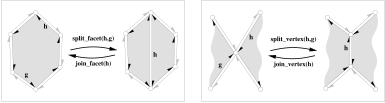
\includegraphics[width=\textwidth]{idraw/euler.ips}%
      }
    \end{center}
\end{ccTexOnly}

\begin{ccHtmlOnly}
    <CENTER>
    <img src="./euler_facet.gif" alt="Euler Facet Operator"><P>
    </CENTER>
\end{ccHtmlOnly}

\ccMethod{Halfedge* split_facet( HDS& hds, Halfedge* h, Halfedge* g);}
    {splits the facet incident to \ccc{h} and \ccc{g} into two facets
     with a new diagonal between the two vertices denoted by \ccc{h} and
     \ccc{g} respectively. The second (new) facet  obtained from
     \ccc{hds} is a copy of the first facet. The new diagonal is
     returned. The time is proportional to the distance from \ccc{h} 
     to \ccc{g} around the facet.
     \ccPrecond \ccc{g} must be reachable from \ccc{h} around the 
     facet.} 

\ccMethod{Halfedge* join_facet( HDS& hds, Halfedge* h);}
    {joins the two facets incident to $h$. The facet incident to
      \ccc{h->opposite()} gets removed by \ccc{hds}. Both facets might be
    holes. Returns the predecessor of $h$ around the facet. The invariant
    \ccc{join_facet( split_facet( h, g))} returns $h$ and keeps
    the data structure unchanged. The time is proportional to the size
    of the facet removed and the time to compute \ccc{h->prev()}.
    \ccPrecond \ccc{HDS} supports removal of halfedges and facets.}


\begin{ccHtmlOnly}
    <CENTER>
    <img src="./euler_vertex.gif" alt="Euler Vertex Operator"><P>
    </CENTER>
\end{ccHtmlOnly}

\ccMethod{Halfedge* split_vertex( HDS& hds, Halfedge* h, Halfedge* g);}
    {splits the vertex incident to \ccc{h} and \ccc{g} into two vertices
     and connects them with a new edge. The second (new) vertex
     obtained from \ccc{hds} is a copy of the first vertex. The
     new edge is returned. The time is proportional to the distance
     from \ccc{h} to \ccc{g} around the vertex.
     \ccPrecond \ccc{g} must be reachable from \ccc{h} around the 
     vertex.} 

\ccMethod{Halfedge* join_vertex( HDS& hds, Halfedge* h);}
    {joins the two vertices incident to $h$. The vertex denoted by
     \ccc{h->opposite()} gets removed by \ccc{hds}. Returns the predecessor of
     $h$ around the vertex. The invariant 
     \ccc{join_vertex( split_vertex( h, g))} returns $h$
     and keeps \ccc{hds} unchanged. 
     The time is proportional to the degree of the vertex removed and 
     the time to compute \ccc{h->prev()}.
     \ccPrecond \ccc{HDS} supports removal of vertices and halfedges.}

\begin{ccTexOnly}
    \begin{center}
      \parbox{0.636\textwidth}{%
          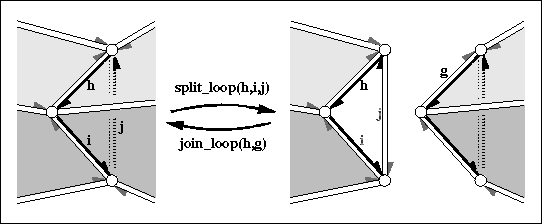
\includegraphics[width=0.636\textwidth]{idraw/euler_loop.ips}%
      }
    \end{center}
\end{ccTexOnly}

\begin{ccHtmlOnly}
    <CENTER>
    <img src="./euler_loop.gif" alt="Euler Loop Operator"><P>
    </CENTER>
\end{ccHtmlOnly}

\ccMethod{Halfedge* split_loop( HDS& hds, 
                                Halfedge* h, Halfedge* i, Halfedge* j);}
   {cuts the halfedge data structure into two parts along the cycle $(h,i,j)$.
    Three new vertices (one copy for each vertex in the cycle) and
    three new halfedges (one copy for each halfedge in the cycle), and
    two new triangles will be 
    created. $h,i,j$ will be incident to the first new triangle.
    The return value will be a halfedge denoting the
    new halfedge of the second new triangle which was \ccc{h-opposite()}
    beforehand.
    \ccPrecond $h,i,j$ are distinct, consecutive vertices of the
    halfedge data structure and form a cycle: i.e. \ccc{h->vertex() ==
    i->opposite()->vertex()}, \ldots, \ccc{j->vertex() ==
    h->opposite()->vertex()}.}

\ccMethod{Halfedge* join_loop( HDS& hds, Halfedge* h, Halfedge* g);}
   {glues the boundary of two facets together.
    Both facets and the vertices of the facet loop $g$ gets removed. 
    Returns $h$. Both facets might be holes.  
    The invariant \ccc{join_loop( h, split_loop( h, i, j))} 
    returns  $h$ and keeps the data structure unchanged.
    \ccPrecond \ccc{HDS} supports removal of vertices, halfedges, and facets.
    The facets denoted by $h$ and $g$ are different and have an
    equal degree (i.e.~number of edges).} 


% -----------------------------------------
\ccHeading{Modifying Functions (Primitives)}

\ccThree{void}{D.set_facet_halfedge( Facet* f, Halfedge* g)}{}

\ccMethod{void set_point( Vertex* v, const Point& p);}{sets the
    point of $v$ to $p$.}
\ccGlue
\ccMethod{void set_point( Halfedge* h, const Point& p);}{sets the
    point of the vertex incident to $h$ to $p$.}
\ccGlue
\ccMethod{void set_vertex_halfedge( Vertex* v, Halfedge* g);}{sets the
    incident halfedge of $v$ to $g$.}
\ccGlue
\ccMethod{void set_vertex_halfedge( Halfedge* h);}{sets the incident
    halfedge of the vertex incident to $h$ to $h$.}

\ccMethod{void set_vertex( Halfedge* h, Vertex* v);}{sets the incident
    vertex of $h$ to $v$.}
\ccGlue
\ccMethod{void set_prev( Halfedge* h, Halfedge* g);}{sets the previous
  link of $h$ to $g$.}
\ccGlue
\ccMethod{void set_facet( Halfedge* h, Facet* f);}{sets the incident
  facet of $h$ to $f$.}
\ccGlue
\ccMethod{void set_facet_halfedge( Facet* f, Halfedge* g);}{sets the
  incident halfedge of $f$ to $g$.}
\ccGlue
\ccMethod{void set_facet_halfedge( Halfedge* h);}{sets the incident
  halfedge of the facet incident to $h$ to $h$.}


% -----------------------------------------
\ccHeading{Miscellaneous}
\ccThree{void}{D.is_val}{}

\ccMethod{bool is_valid( const HDS& hds, bool verbose = false, 
    int level = 0) const;}{%
    returns \ccc{true} if the halfedge data structure \ccc{hds} is
    valid with respect to the \ccc{level} value. If \ccc{verbose} is
    \ccc{true}, statistics are printed to \ccc{cerr}. A halfedge data
    structure has no definition of validness of its own, but a useful
    set of tests is defined with the following levels:
    \\[6pt]
    {\em Level 0:} The number of halfedges is even. All pointers
    except the facet pointer for border halfedges are unequal to
    \ccc{NULL}. For all halfedges $h$: The opposite halfedge is
    different from $h$ and the opposite of the opposite is equal to
    $h$. The next of the previous halfedge is equal to $h$. For all
    vertices $v$: the incident vertex of the incident halfedge of $v$
    is equal to $v$. The halfedges around $v$ starting with the
    incident halfedge of $v$ form a cycle.  For all facets $f$: the
    incident facet of the incident halfedge of $f$ is equal to $f$.
    The halfedges around $f$ starting with the incident halfedge of
    $f$ form a cycle.  Some checks that redundancies among internal
    variables holds, e.g. that the iterators enumerate as many items
    as the related size value indicates.
    \\[6pt]
    {\em Level 1:} All tests of level 0. For all halfedges $h$: The
    incident vertex of $h$ is equal to the incident vertex of the
    opposite of the next halfedge. The incident facet of $h$ is equal
    to the incident facet of the next halfedge.
    \\[6pt]
    {\em Level 2:} All tests of level 1. The sum of all halfedges that
    can be reached through the vertices must be equal to the number of
    all halfedges, i.e.~all halfedges incident to a vertex must form a
    single cycle.
    \\[6pt]
    {\em Level 3:} All tests of level 2. The sum of all halfedges that
    can be reached through the facets must be equal to the number of
    all halfedges, i.e.~all halfedges surrounding a facet must form a
    single cycle (no holes in facets).
    \\[6pt]
    {\em Level 4:} All tests of level 3 and
    \ccc{normalized_border_is_valid}.  }

\ccMethod{bool normalized_border_is_valid( const HDS& hds, 
  bool verbose = false) const;}{%
    returns \ccc{true} if the border halfedges are in normalized 
    representation, which is when enumerating all halfedges with the
    iterator: The non-border edges precede the border edges. For
    border edges, the second halfedge is a border halfedge. (The first
    halfedge may or may not be a border halfedge.) The halfedge
    iterator \ccc{border_halfedges_begin()} denotes the first border
    edge. If \ccc{verbose} is \ccc{true}, statistics are
    printed to \ccc{cerr}.
}


\end{ccClassTemplate}



% +========================================================================+
\clearpage
\section{Examples of Halfedge Data Structures}
% +========================================================================+
\label{sectionHdsExamples}


% +-------------------------------------------------------------+
\subsection{The Default Halfedge Data Structure}

The default halfedge data structure from
Section~\ref{sectionHdsDefault} expects a point as template argument,
which we choose to be an {\tt int} for simplicity. The example program
defines a halfedge data structure and a decorator, see
Section~\ref{sectionHdsDecorator} for the decorator. The program
creates a loop, consisting of two halfedges, one vertex and two
facets, and checks its validity.

\ccIncludeVerbatim{hds_prog_default.C}


% +-------------------------------------------------------------+
\subsection{A Minimal Halfedge Data Structure}

The following program declares a minimal structure {\tt HDS} using the
minimal bases provided in Section~\ref{sectionHdsBasesModels} and a
list-bases halfedge data structure from
Section~\ref{sectionHdsUsingList}. The result is a data structure
maintaining only halfedges with next and opposite pointers.  No
vertices or facets are stored. The data structure models an {\em
  undirected graph}.

\ccIncludeVerbatim{hds_prog_graph.C}


% +-------------------------------------------------------------+
\subsection{The Default with a Vector Instead of a List}

The default halfedge data structure uses a list internally and the
maximal base classes. Assuming we have a point type {\tt Point} we can
declare an alternative data structure {\tt HDS} using the same base
classes but the vector storage from Section~\ref{sectionHdsUsingVector}.
Note that for the vector storage the size of the halfedge data
structure must be reserved beforehand, either with the constructor as
shown in the example or with the {\tt reserve()} member function.

\ccIncludeVerbatim{hds_prog_vector.C}


% +-------------------------------------------------------------+
\subsection{Example Adding Color to Facets}

This example re-uses the base class available for facets and adds
another member variable \ccc{color}. The facet in the halfedge data
structure and data structures building upon that will inherit 
the new member variable, as the main function indicates. The same can
be done with any kind of functionality and any of the three items;
vertices, halfedges or facets. However, note that additional pointers
to vertices, halfedges, and facets cannot be introduced this way,
since they are only maintained as {\tt void*} pointers at this
level. The internal classes, which are responsible for the type safe
pointers, must be extended to achieve this.

\ccIncludeVerbatim{hds_prog_color.C}


% +-------------------------------------------------------------+
\subsection{Example Extending the Minimal Halfedge Base with a
  Previous Pointer}

The minimal halfedge data structure above can be extended to a data
structure also supporting a previous pointer for halfedges. We replace
the \ccc{Halfedge_min_base} with our own \ccc{Halfedge_base}
derived from the \ccc{Halfedge_min_base}.

\begin{verbatim}
  class My_halfedge : public Halfedge_min_base {
      void* prv;
  public:
      typedef  Tag_true   Supports_halfedge_prev;
      void*       prev()                    { return prv;}
      const void* prev() const              { return prv;}
      void        set_prev( void* h)        { prv = h;}
  };  
\end{verbatim}

% +-------------------------------------------------------------+
\subsection{Example Using own Halfedge Structure}

\begin{ccAdvanced}
  
The halfedge data structure as presented here is not as space efficient as
for example the winged
edge data structure~\cite{b-prcv-75}, the DCEL~\cite{mp-fitcp-78} or
variants of the quad-edge data structure~\cite{gs-pmgsc-85}.
On the other side they do not need any search operations during
traversals. A comparison can be found in~\cite{k-ddsps-98}.

Computation time versus memory space can also be traded with the
halfedge data structure design as presented here.  We will use
traditional C techniques like type casting and make the assumption
that pointers (especially those from {\tt malloc} or {\tt new}) points
to even addresses. The idea is as follows: The halfedge data structure
allocate halfedges pairwise.  Concerning the vector based data
structure this implies that the absolute value of the difference
between a halfedge and its opposite halfedge is always one with
respect to C pointer arithmetic. We can replace the opposite pointer
by a single bit coding the sign of this difference.  We will store
this bit as the least significant bit together with the next halfedge
pointer.  The example also omits the previous pointer. What remains
are three pointers per halfedge. The same solution can be applied to
the list based polyhedron traits class with the difference that the
{\tt SIZE} constant must reflect the additional pointers needed for
the list management. They are added internally of the halfedge data
structure using the base class \ccc{In_place_list_base<My_halfedge>}.


\ccIncludeVerbatim{hds_prog_compact.C}

\end{ccAdvanced}

% +-------------------------------------------------------------+
\subsection{Example Using the Halfedge Iterator}

Three edges are created in the default halfedge data structure.
The halfedge iterator is used to count the halfedges.

\ccIncludeVerbatim{hds_prog_halfedge_iterator.C}

% +-------------------------------------------------------------+
\subsection{Example for an Adaptor to Build an Edge Iterator}

Three edges are created in the default halfedge data structure.
The adaptor {\tt N\_step\_adaptor} is used to declare an edge
iterator, which is used to count the edges.

\ccIncludeVerbatim{hds_prog_edge_iterator.C}

% +--------------------------------------------------------+

% EOF
